\section{Weiterentwicklung}

In der zweiten Phase des Projekts soll die Funktionalität des KSM erweitert werden. Besonderes Augenmerk liegt hierbei auf der Verbesserung der Anzeige, welche Knoten im aktiven/passiven, oder kritischen Bereich liegen. Diese Anzeige wird im KSM Projekt auch Sum-Chart genannt. Hier wurde bereits in einer der letzten Studienarbeiten von Frau Klein angefangen es dem Benutzer zu ermöglichen Bereiche zu definieren und zu markieren \cite{bib:klein}. Bereiche waren in diesem Fall Ellipsen, die vom Benutzer aufgezogen wurden. Je größer diese wurden, desto transparenter wurde die Füllfarbe. Die Abbildung \ref{ellipse} zeigt den letzten Stand dieser Implementierung.
\begin{figure}[h]
	\centering
	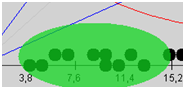
\includegraphics[width=0.6\textwidth]{pictures/ellipse.png}
	\caption{Bereichsmarkierung nach Klein \cite{bib:klein}}
	\label{ellipse}
\end{figure}

Nach Evaluation dieser Implementierung kam Herr Professor Schubert zu dem Schluss, dass Ellipsen auf der einen Seite zu unflexibel sind, um einen Bereich adäquat ausbilden zu können. Auf der anderen Seite jedoch auf keinerlei Begrenzungen, wie zum Beispiel aktiv/passiv-Geraden  Rücksicht nehmen. Außerdem wurde die Füllfarbe trotz Transparenz teilweise als zu deckend empfunden.

\subsection{Anforderungen}

Die neuen Anforderungen an eine Bereichsmarkierung lauteten nach diesen Erkenntnissen wie folgt:
\begin{itemize}
  \item Der Benutzer muss in der Lage sein, einen Bereich mittels Eckpunkten definieren zu können
  \item Es muss möglich sein, eine beliebige Anzahl an Eckpunkten eingeben zu können
  \item Die Eckpunkte dürfen nur auf bereits vorhandenen Linien gesetzt werden:
  \begin{itemize}
    \item X-Achse
    \item Y-Achse
    \item Q-Achsen zur Abgrenzung der aktiven/passiven Bereiche, sowie Q = 1 als Mitte
    \item Hyperbeln zur Markierung des stabilen/kritischen Bereichs
  \end{itemize}
  \item Punkte (Knoten des System Graphen), die innerhalb des markierten Bereichs liegen, müssen aufgelistet werden
  \item Die Füllfarbe des Bereichs soll transparenter sein, als bisher
\end{itemize}

Dazu wurde noch von den Projektmitgliedern entschieden, dass erstellte Bereiche benannt werden sollen. Dieser Name soll innerhalb des Bereichs sichtbar sein.

\subsection{Ergebnis}

Die gestellten Anforderungen wurden vollständig umgesetzt. Der Benutzer kann nun durch Setzen mehrerer Eckpunkte, die sich auf den vorgegebenen Linien befinden ein Polygon definieren.

Damit der Benutzer immer weiß, wo der nächste Eckpunkt gesetzt werden würde, ist ein roter Punkt implementiert worden, der sich immer auf dem entsprechenden Punkt der zur Mauspostion nächsten gültigen Linie befindet und so den nächsten Eckpunkt markiert (Abbildung \ref{roterPunkt}).
\begin{figure}
	\centering
	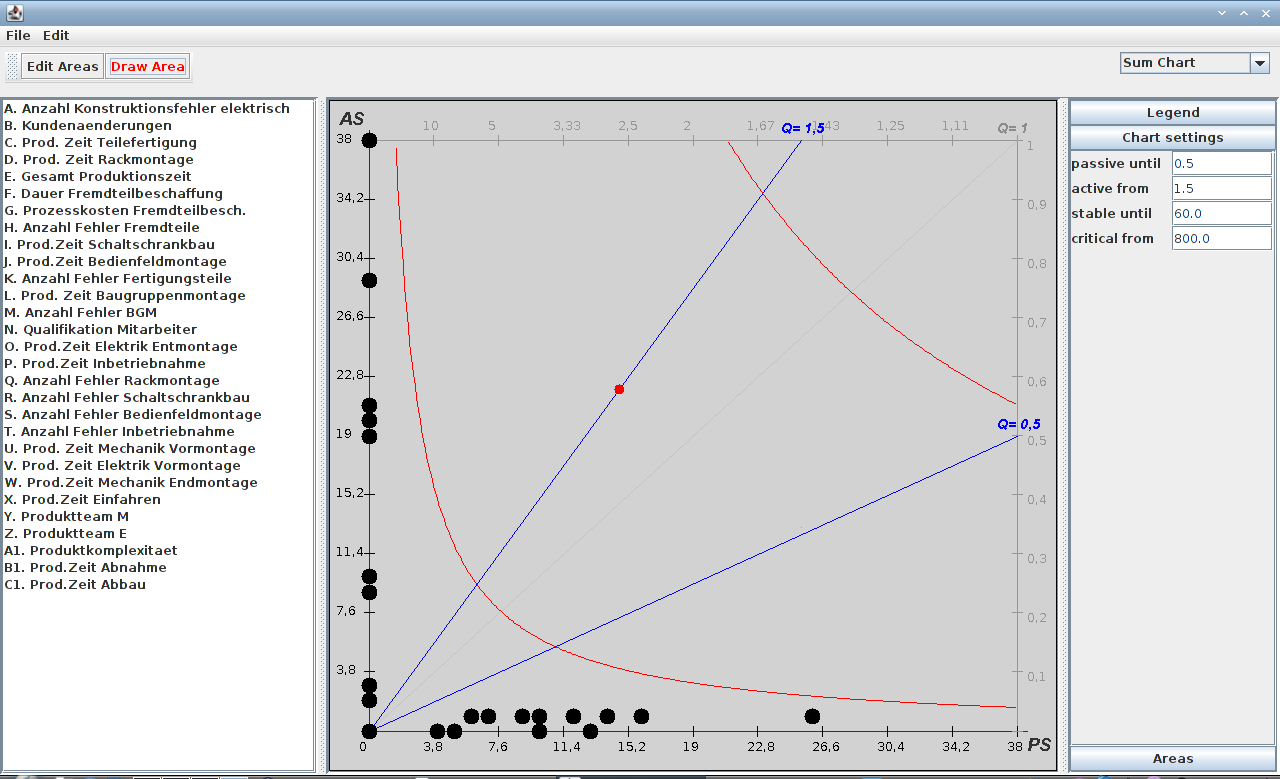
\includegraphics[width=1\textwidth]{pictures/roter-punkt.png}
	\caption{roter Punkt}
	\label{roterPunkt}
\end{figure}

Mittels Klick wird der Punkt gespeichert und ein vorläufiges Polygon gezeichnet. Will der Benutzer die Eingabe beenden, kann er das Polygon mit einem Doppelklick abschließen. Anschließend wird ein Auswahldialog präsentiert, der dem Benutzer die Möglichkeit eröffnet, das Polygon zu übernehmen, oder zu verwerfen.
Abbildung \ref{menü} zeigt ein abgeschlossenes Polygon und das Auswahlmenü.
\begin{figure}
	\centering
	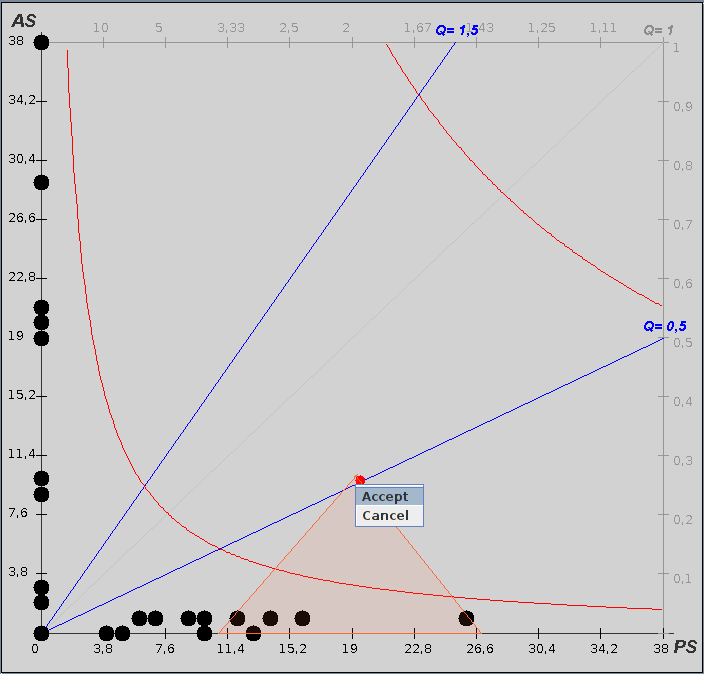
\includegraphics[width=0.8\textwidth]{pictures/menu.png}
	\caption{abgeschlossenes Polygon mit Auswahldialog}
	\label{menü}
\end{figure}

Nachdem ein Polygon akzeptiert und benannt wurde, ermittelt das Programm, welche Knoten sich innerhalb dieses Polygons befinden und listet diese in einer Baumstruktur auf. Diese Auflistungen können im rechten Panel unter dem Eintrag ,,Areas'' gefunden werden. Abbildung \ref{baum} zeigt diese Auflistung für das Polygon ,,Beispiel''.
\begin{figure}
	\centering
	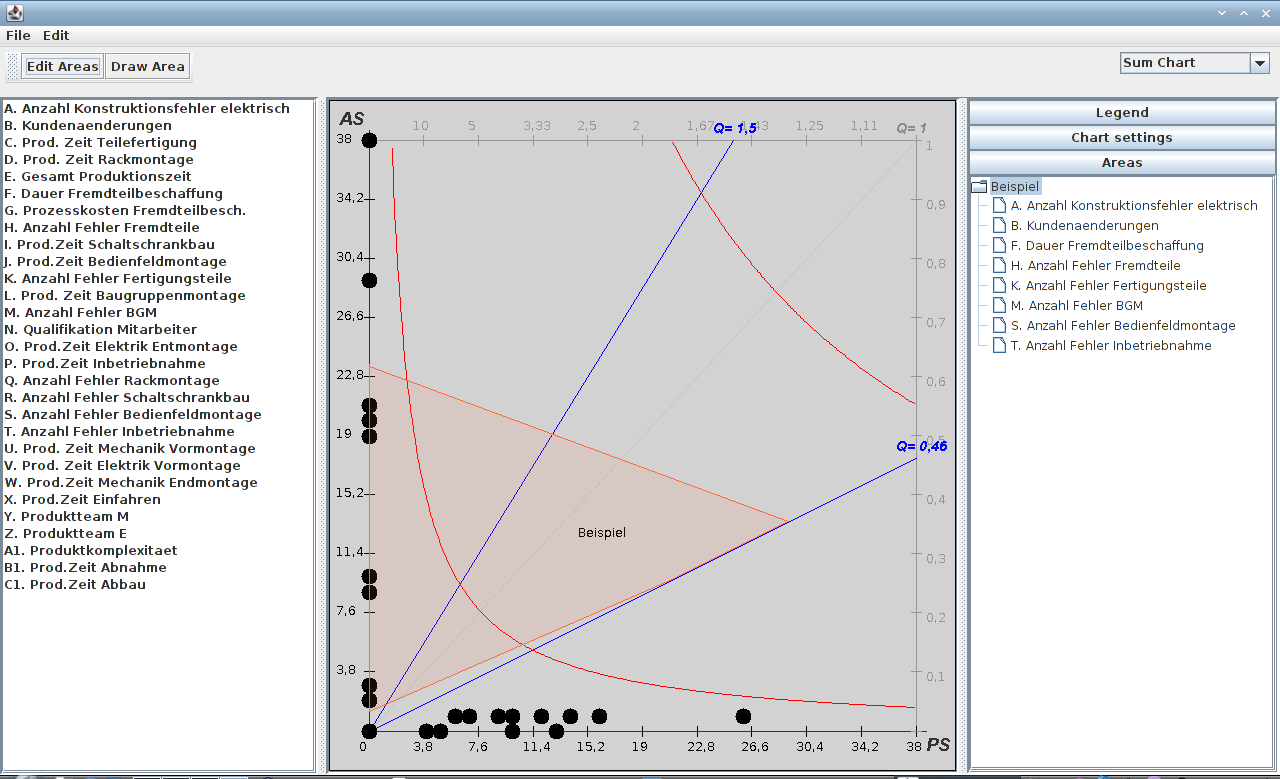
\includegraphics[width=1\textwidth]{pictures/baum.png}
	\caption{Baumdarstellung der Knoten innerhalb eines Polygons}
	\label{baum}
\end{figure}

Die Anforderung der zu geringen Transparenz wurde etwas anders gelöst, als anfangs geplant. Die ursprüngliche Implementierung von Frau Klein sah vor, dass die Transparenz mit der Größe der Fläche zunimmt. Dieser Umstand führte in der neuen Implementierung dazu, dass obwohl der Transparenzwert erhöht wurde, kleine Flächen immer noch viel zu deckend, große Flächen jedoch kaum noch sichtbar waren. Deswegen wurde die Kopplung der Transparenz mit der Fläche aufgehoben und stattdessen eine starke Transparenz der Füllfarbe definiert und die Fläche zudem mit einer deckenden Umrandung versehen. Dies ermöglicht eine gute Sichtbarkeit der Knoten und Werte innerhalb des Polygons, bei gleichzeitiger guter Sichtbarkeit des Polygons selbst, wie auf den Abbildungen \ref{menü} und \ref{baum} zu sehen ist.



\subsection{Implementierung}

Die Implementierung der neuen Funktionalitäten lässt sich in mehrere Aspekte unterteilen.
\begin{enumerate}
\item Ausprogrammieren der gültigen Linien
\item Ermittlung der nächsten gültigen Linie zur Mausposition
\item Zeichnen des aktuellen Polygons
\item Speicherung und Anzeige akzeptierter Polygone
\item Ermittlung der Punkte innerhalb eines Polygons und Darstellung in einem Baum
\end{enumerate}

Da diese Aufgabe im Team mit Herr Vogt gelöst werden sollte, wurden die Aspekte aufgeteilt. Herr Vogt bearbeitete Aspekt Nr. 1, ich die Aspekte 2 - 5. Im folgenden sollen nun die wichtigsten Details meiner Implementierungen erläutert werden.

\begin{description}
\item[Ermittlung der nächsten gültigen Linie zur Mausposition:] Um die nächste Linie zu ermitteln wurde ein Interface definiert, das alle Klassen, die eine Linie repräsentieren implementieren müssen. Anhand dieses Interfaces kann gesammelt über alle Linien des Diagramms iteriert und Funktionswerte verglichen werden. Listing \ref{function} zeigt die Definition des Interfaces.
\begin{lstlisting}[captionpos=b, caption=Interface für die Linien, label=function]
public interface Function {
    public Point calcY(int x, int y);
}
\end{lstlisting}

Wie in Listing \ref{function} zu sehen, wird immer ein Punkt zurückgegeben. Dieser Punkt definiert den Punkt auf der Linie, der am ehesten der aktuellen Mausposition entsprechen würde. Diese Punkte können nun verglichen werden.
\begin{lstlisting}[captionpos=b, caption=Methode zum ermitteln des nächsten Punktes, label=setPoint]
Point bestPoint = new Point();
        int bestDist = 1000000;
        for (Function function : functions) {
            Point curPoint = function.calcY(x, y);

            int dist = Math.abs(x - curPoint.x) + Math.abs(y -curPoint.y);
            if(dist < bestDist){
                bestDist = dist;
                bestPoint = curPoint;
            }
        }
\end{lstlisting}

Listing \ref{setPoint} zeigt die Ermittlung der nächsten Linie. Der Abstand des Punktes auf der Linie zur aktuellen Mausposition wird durch die Addition der absoluten Abstände der X- und Y-Werte berechnet. Ist dieser Abstand kleiner als der bisherige kleinste Abstand, so wird dieser übernommen und der Punkt gespeichert. 

Damit diese Methode bei jeder Mausbewegung aufgerufen wird, ist es noch notwendig einen eigenen MouseMotionListener zu implementieren. Dieser reagiert auf Ereignisse, die durch die Maus zum Beispiel beim Bewegen ausgelöst werden. Dieser MouseMotionListener ist in Listing \ref{mmlistener} abgebildet. Dort wird bei jeder Mausbewegung die Methode \emph{setPoint} aufgerufen, die die Berechnung aus Listing \ref{setPoint} beinhaltet. Im Anschluss wird das gesamte Bild neu gezeichnet.
\begin{lstlisting}[captionpos=b, caption=MouseMotionListener, label=mmlistener]
class drawAreaMouseMotionListener extends MouseMotionAdapter{
        @Override
        public void mouseMoved(MouseEvent event){
            setPoint(event.getX(), event.getY());
            repaint();
        }
}
\end{lstlisting}

\item[Zeichnen des aktuellen Polygons:] Das aktuelle Polygon muss immer dann neu gezeichnet werden, wenn der Benutzer durch einen Klick einen neuen Eckpunkt hinzufügt. Um diesen Klick zu registrieren, muss wieder ein MouseListener implementiert werden. Dieser reagiert allerdings nicht auf Mausbewegungen, wie der vorherige MouseListener, sondern auf Klicks. Somit wird in der Methode \emph{mouseClicked} der im vorherigen Schritt ermittelte Punkt zu dem aktuellen Polygon hinzugefügt (Listing \ref{addPoint}).
\begin{lstlisting}[captionpos=b, caption=Neuen Punkt zum Polygon hinzufügen, label=addPoint]
polygon.addPoint(currentPoint.x, currentPoint.y);
repaint();
\end{lstlisting}

Mit dem Aufruf der Methode \emph{repaint} wird unter anderem die Methode \emph{paint} ausgeführt. Dort wird das Polygon neu gezeichnet.
\begin{lstlisting}[captionpos=b, caption=Zeichnen des Polygons, label=drawPol]
g.setColor(ovalColor[2-x_index][2-y_index]);
g.drawPolygon(polygon);

Composite c = AlphaComposite.getInstance(AlphaComposite.SRC_OVER,0.1f);
g2d.setComposite(c);

g.fillPolygon(polygon);
\end{lstlisting}

In Listing \ref{drawPol} wird die Zeichenroutine aufgeführt. Es ist zu sehen, dass zuerst mit der Methode \emph{drawPolygon} nur die Umrisse des Polygons gezeichnet werden. Anschließend wird der Alphakanal verändert, um die Transparenz der Farbe zu beinflussen, damit die Füllung des Polygons die darunterliegenden Knoten nicht überdeckt.

\item[Speicherung und Anzeige akzeptierter Polygone:] Die Definition eines neuen Polygons wird mit einem Doppelklick abgeschlossen. Dieser Doppelklick wird ebenfalls mit dem vorherigen MouseListener registriert. Daraufhin wird dem Benutzer ein Dialog präsentiert, in dem er wählen kann, ob das Polygon gespeichert, oder verworfen werden soll. Soll das Polygon behalten werden, ist vom Benutzer ein Name zu vergeben. Listing \ref{speichern} zeigt, wie die Speicherroutine implementiert wurde.
\begin{lstlisting}[captionpos=b, caption=Routine zum Speichern eines Polygons, label=speichern]
String description = JOptionPane.showInputDialog(parent, "Give in a description..", "Area Description", 3);
if(description == null){
  polygon = new Polygon();
  repaint();
  return;
}  
NamedPolygon pol = new NamedPolygon(polygon.xpoints, polygon.ypoints, polygon.npoints);
pol.setName(description);
searchInnerPoints(pol);
polygons.add(pol);
polygon = new Polygon();
repaint();
\end{lstlisting}

Die Zeilen 1 - 6 Erzeugen einen Eingabedialog für den Namen. Gibt der Benutzer keinen Namen ein, wird die Routine abgebrochen. Im Anschluss wird ein neues Polygon vom selbst erzeugten Typ NamedPolygon (Listing \ref{namedP}) instanziiert, dem der vom Benutzer eingegebene Name zugewiesen wird. Daraufhin wird das neue Polygon in einer Liste gespeichert und das alte Polygon wieder zurückgesetzt. 
\begin{lstlisting}[captionpos=b, caption=Klassendefinition des NamedPolygon, label=namedP]
public class NamedPolygon extends Polygon{
    String name;

    public NamedPolygon(int xpoints[], int ypoints[], int npoints){
        super(xpoints, ypoints, npoints);
    }
    public NamedPolygon(){
        super();
    }
    public void setName(String name){
        this.name = name;
    }
    public String getName(){
        return this.name;
    }

}
\end{lstlisting}

\item[Ermittlung der Punkte innerhalb eines Polygons und Darstellung in einem Baum:] In Zeile 9 des Listings \ref{speichern} wird die Methode \emph{searchInnerPoints} bereits aufgerufen. Listing \ref{siPoints} zeigt diese Methode.
\begin{lstlisting}[captionpos=b, caption=Methode searchInnerPoints, label=siPoints]
public void searchInnerPoints(NamedPolygon pol){
        DefaultMutableTreeNode root = new DefaultMutableTreeNode(pol.getName());
        List<String> innerPoints = new ArrayList<String>();
        for(int i=0; i<points.size();i++){
            if(pol.contains(points.elementAt(i))){
                String name = data.getListModelNodes().getElementAt(i).toString();
                innerPoints.add(name);
                DefaultMutableTreeNode child = new DefaultMutableTreeNode(name,false);
                root.add(child);
            }
        }
        
        data.getPolyModel().insertNodeInto(root, data.getRoot(), 0);
}
\end{lstlisting}

In der Methode \emph{searchInnerPoints} geschieht allerdings noch mehr, als nur das ermitteln der Punkte, die innerhalb eines Polygons liegen. Es wird außerdem gleich ein kleiner Teilbaum generiert, in dem das Polygon  selbst die Wurzel und die Knoten Blätter darstellen. Dieser Baum wird an eine externe Klasse übergeben, die in Anlehnung an die Model-View-Controller Architektur als Model fungiert und die Daten der Anzeige beinhaltet. Dieses Model wird nun in einer anderen Anzeige ebenfalls übernommen und der Baum angezeigt. Für diese Anzeige wurde ein weiterer Eintrag im rechten Panel implementiert. Die Klasse \emph{PolyTree} implementiert wie in Listing \ref{polytree} dargestellt das Interface \emph{RightPanelMenuEntry} und kann so in das in der ersten Studienarbeit implementierte Anzeige-Framework eingebettet werden.
\begin{lstlisting}[captionpos=b, caption=Klasse PolyTree, label=polytree]
public class PolyTree implements RightPanelMenuEntry{

    private DataModel model;
    private JPanel pane;
    JScrollPane scPane;
    JTree tree;

    public PolyTree(DataModel model) {
        this.model = model;        
    }

    public String getName() {
        return "Areas";
    }

    public JPanel getPanel() {
        pane = new JPanel();
        scPane = new JScrollPane();
        pane.setLayout(new BoxLayout(pane, BoxLayout.PAGE_AXIS));
        tree = model.getPolygonTree();
        tree.setRootVisible(false);
        tree.expandPath(new TreePath(model.getRoot()));
        scPane.setViewportView(tree);
        pane.add(scPane);
        return pane;
    }
}
\end{lstlisting}

Die Klasse \emph{PolyTree} bekommt im Konstruktor die Model-Klasse übergeben und kann aus dieser den Baum zur Anzeige übernehmen. In der vom Interface vorgegebenen Methode \emph{getPanel} wird dem Framework ein Panel übergeben, dass diesen Baum beinhaltet.
\end{description}